\tikzstyle{pic}=[inner sep=0pt]
\tikzstyle{quote}=[fill=gray!30, inner sep=12pt]

\newcommand{\vogels}{
  \node[pic] (vogels) at (0, 0) {
    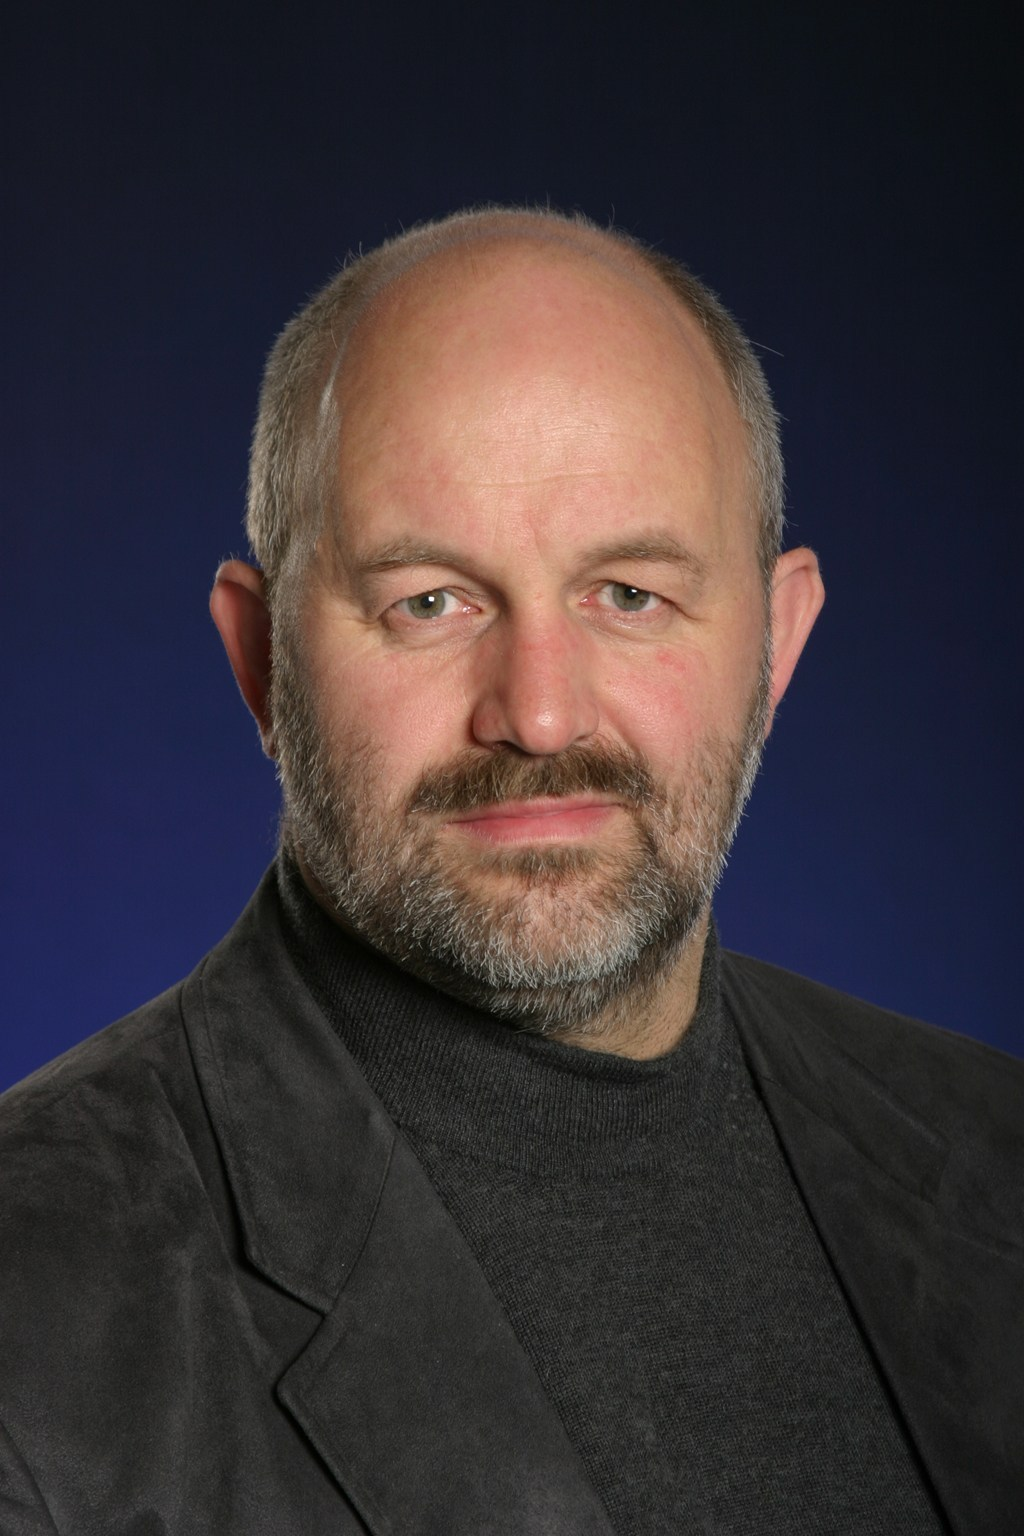
\includegraphics[
      width=0.22\textwidth,
      trim=0 75 0 25,
      clip
    ]{assets/vogels.jpg}
  };
}

\newcommand{\hoare}{
  \node[pic, right=0.2cm of vogels] (hoare) {
    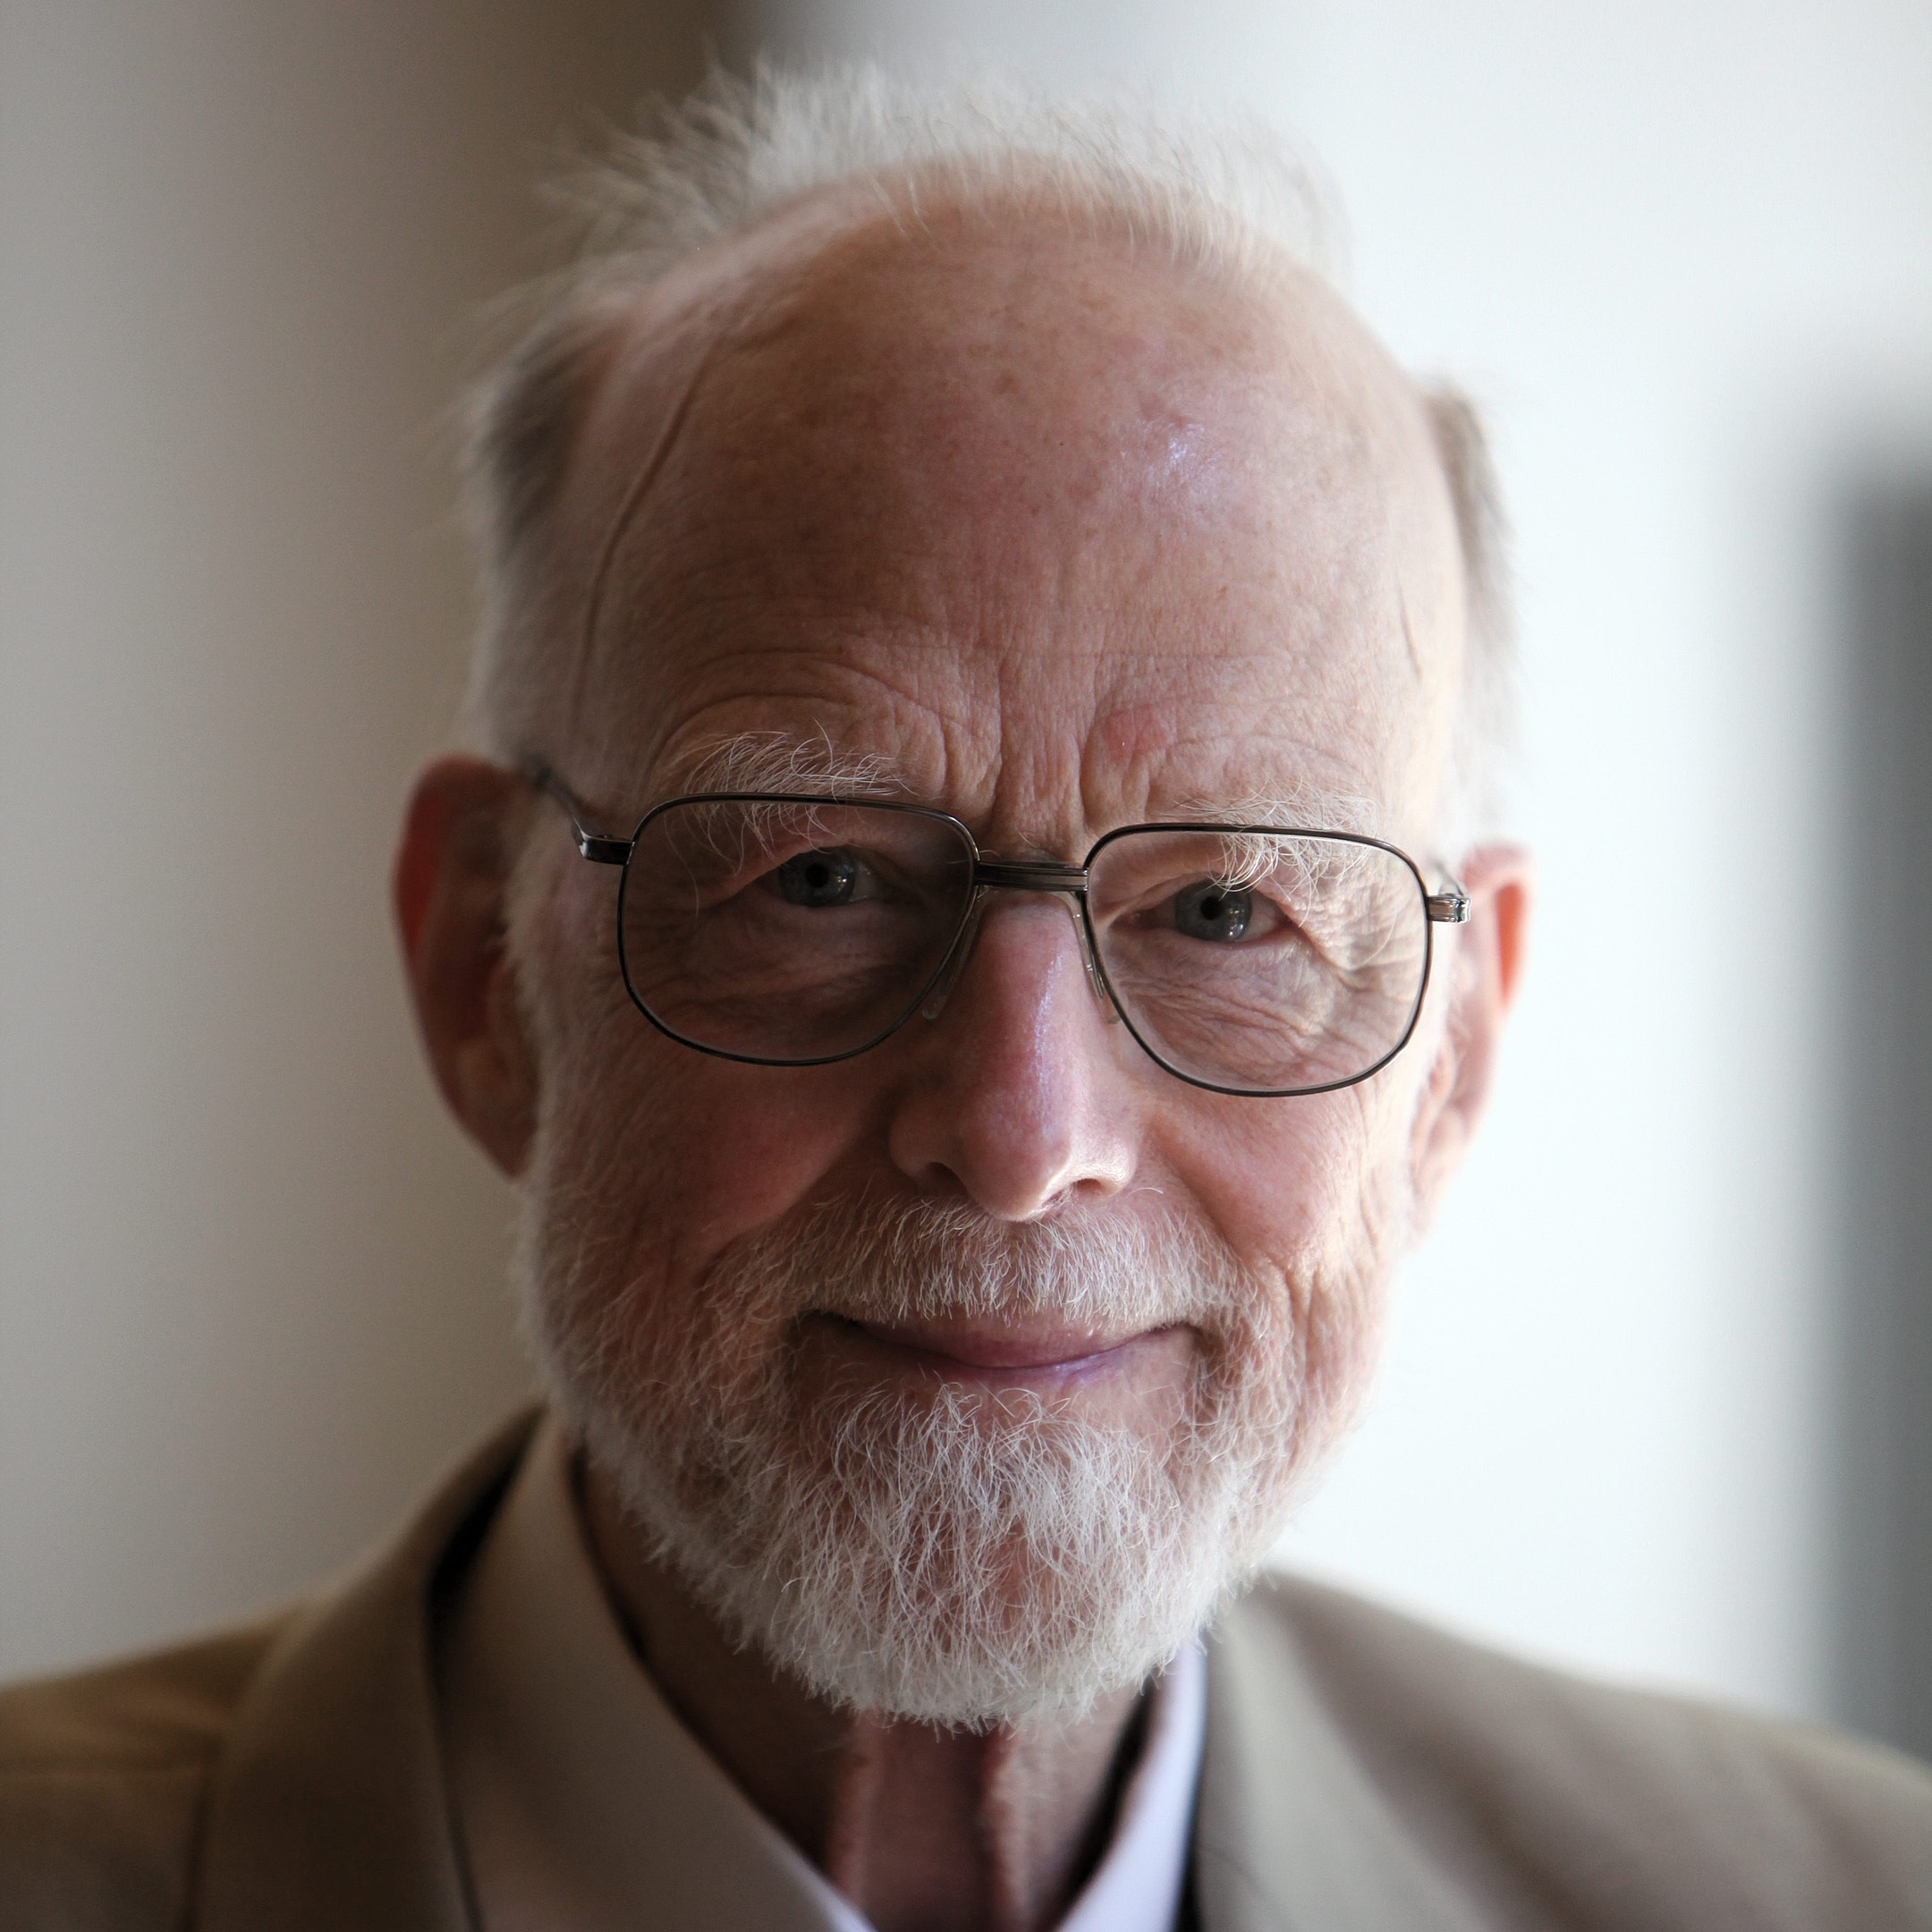
\includegraphics[width=0.22\textwidth]{assets/hoare.jpg}
  };
}

\newcommand{\lamport}{
  \node[pic, right=0.2cm of hoare] (lamport) {
    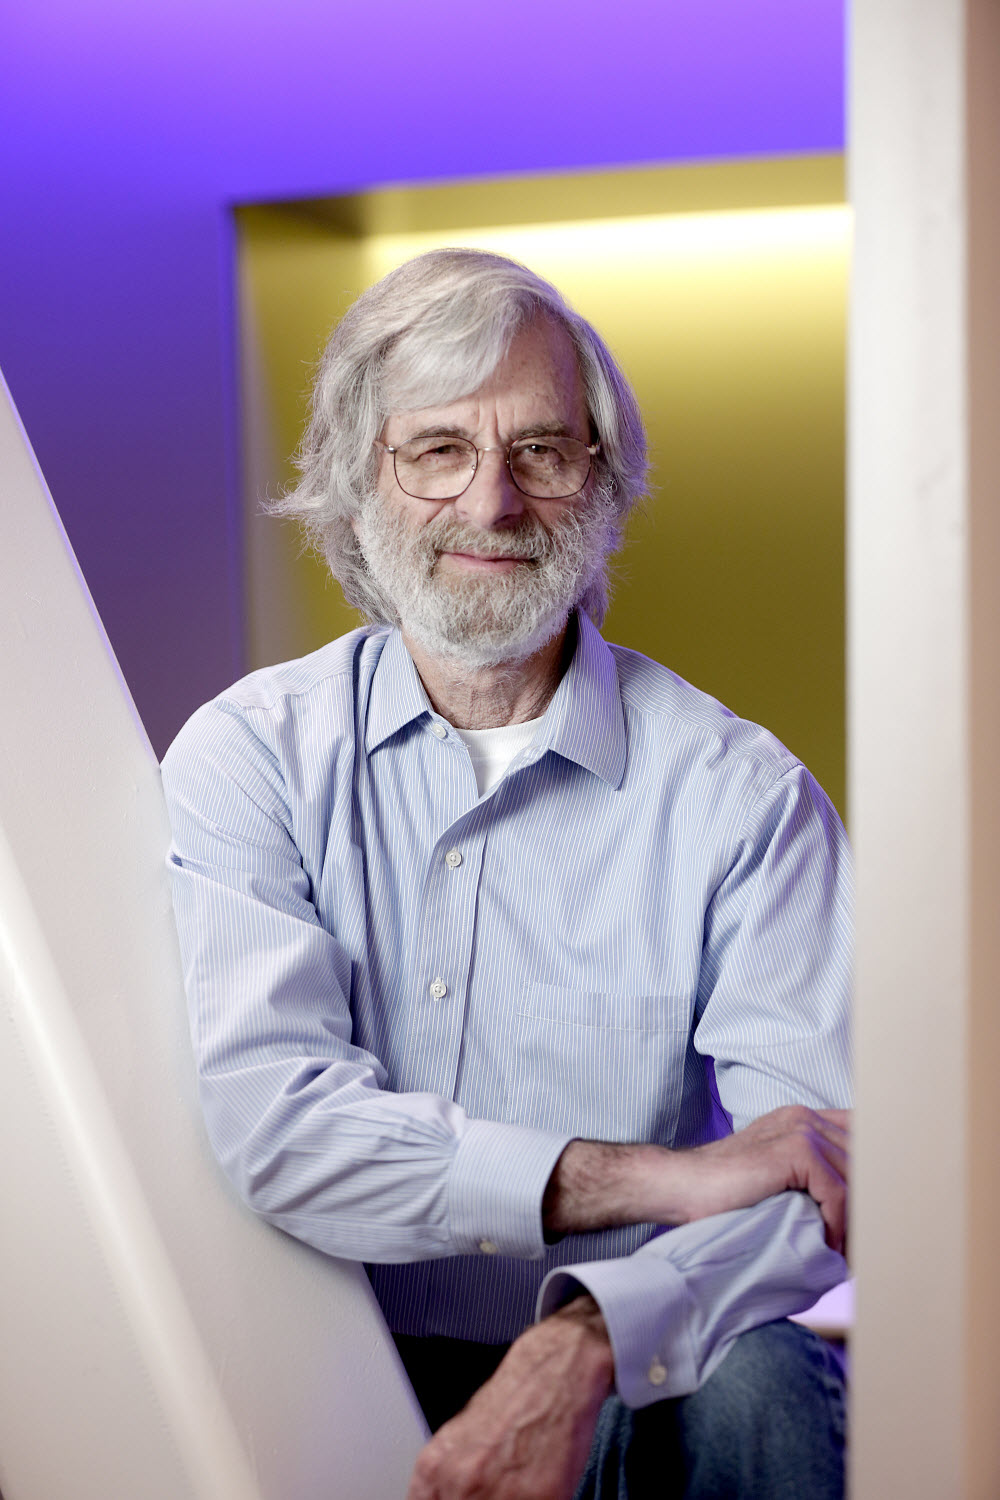
\includegraphics[
      width=0.22\textwidth,
      trim=250 700 300 200,
      clip
    ]{assets/lamport.jpg}
  };
}

\newcommand{\brewer}{
  \node[pic, right=0.2cm of lamport] (brewer) {
    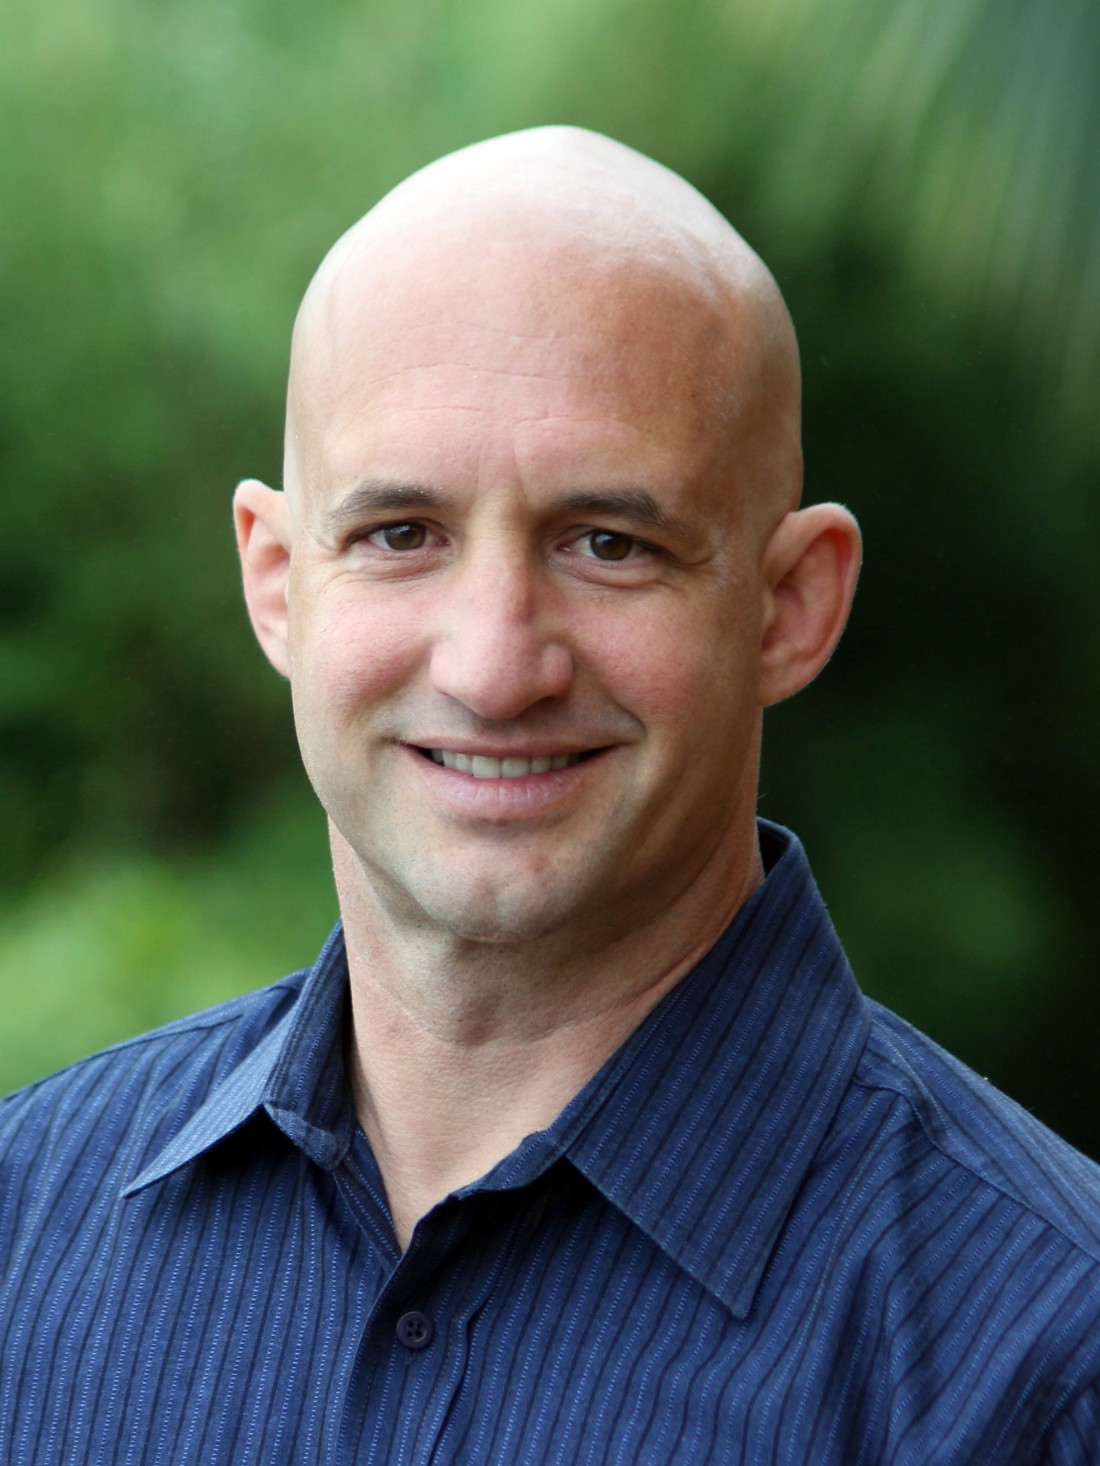
\includegraphics[
      width=0.22\textwidth,
      trim=100 300 100 100,
      clip
    ]{assets/brewer.jpg}
  };
}

\begin{frame}
  \begin{center}
    \begin{tikzpicture}[xscale=1.3]
      \vogels
      \node[quote, text width=0.8\textwidth, align=left] at (0, 3) {
        \Large\textit{You should use weak consistency. It's wicked fast!}
      };
      \path[fill=gray!30] (vogels.north) -- ++(0, 1) -- ++(0.5, 0) -- (vogels.north);
    \end{tikzpicture}
  \end{center}
\end{frame}

\begin{frame}
  \begin{center}
    \begin{tikzpicture}[xscale=1.3]
      \vogels
      \hoare
      \node[quote, text width=0.8\textwidth, align=left] at (1, 3) {
        \Large\textit{What about the application invariants?!}
      };
      \path[fill=gray!30] (hoare.north) -- ++(0, 1.5) -- ++(1, 0) -- (hoare.north);
    \end{tikzpicture}
  \end{center}
\end{frame}

\begin{frame}
  \begin{center}
    \begin{tikzpicture}[xscale=1.3]
      \vogels
      \hoare
      \lamport
      \node[quote, text width=0.8\textwidth, align=left] at (2, 3) {
        \Large\textit{Yeah, go with strong consistency! I have an algorithm for that :)}
      };
      \path[fill=gray!30] (lamport.north) -- ++(0, 1.5) -- ++(1, 0) -- (lamport.north);
    \end{tikzpicture}
  \end{center}
\end{frame}

\begin{frame}
  \begin{center}
    \begin{tikzpicture}[xscale=1.3]
      \vogels
      \hoare
      \lamport
      \brewer
      \node[quote, text width=0.8\textwidth, align=left] at (3, 3) {
        \Large\textit{Not so fast!}
      };
      \path[fill=gray!30] (brewer.north) -- ++(0, 1.5) -- ++(-1, 0) -- (brewer.north);
    \end{tikzpicture}
  \end{center}
\end{frame}

\begin{frame}
  \begin{center}
    \begin{tikzpicture}[xscale=1.3]
      \node[pic] (bailis) at (0, 0) {
\includegraphics[width=0.25\textwidth]{assets/bailis.jpg}};
      \node[quote, text width=0.8\textwidth, align=left] at (0, 3) {
        \Large\textit{?`Porque no los dos?}
      };
      \path[fill=gray!30] (bailis.north) -- ++(0, 1.5) -- ++(1, 0) -- (bailis.north);
    \end{tikzpicture}
  \end{center}
\end{frame}
